% article example for classicthesis.sty
\documentclass[10pt,a4paper]{article} % KOMA-Script article scrartcl
\usepackage{import}
\usepackage{xifthen}
\usepackage{pdfpages}
\usepackage{transparent}
\newcommand{\incfig}[1]{%
    \def\svgwidth{\columnwidth}
    \import{./figures/}{#1.pdf_tex}
}
\usepackage{lipsum}     %lorem ipsum text
\usepackage{titlesec}   %Section settings
\usepackage{titling}    %Title settings
\usepackage[margin=10em]{geometry}  %Adjusting margins
\usepackage{setspace}
\usepackage{listings}
\usepackage{amsmath}    %Display equations options
\usepackage{amssymb}    %More symbols
\usepackage{xcolor}     %Color settings
\usepackage{pagecolor}
\usepackage{mdframed}
\usepackage[english]{babel}
\usepackage[utf8]{inputenc}
\usepackage{longtable}
\usepackage{multicol}
\usepackage{graphicx}
\graphicspath{ {./Images/} }
\setlength{\columnsep}{1cm}

% ====| color de la pagina y del fondo |==== %
\pagecolor{white}
\color{black}



\begin{document}
    %========================{TITLE}====================%
    \title{{  6th laboratory  }}
    \author{{Rodrigo Castillo}}
    \date{\today}

    \maketitle


    %=======================NOTES GOES HERE===================%
%    \section{ Read the introduction of the section 6 "Recognizing C Code
%        Constructs in Assembly" and explain what means a "Code Construct". What
%        aspects may impact the way as assembly code is generated?}
%        \color{red} this section is not supposed to be includded in laboratory \color{black}


%    \section{Read the section "Gobal vs Local Variables" and identify what are
%        the differences in the compilation of a code that employs global vs one
%        that employs local Variables.Ref: Section "Registers" Pag 104, Section "The Stack" Pag 110, Section "Stack
%        Layout" Pag 111. Section "C Main Method and Offsets" Pag 116.}
%        \color{red} this section is not supposed to be includded in laboratory \color{black}

    \section{operations :addition, substraction , increment, decrement and modulo}

        for addition:
        we can see that the addition operation is in line $ 666  $  , in
        operation $ add  $  , as i defined two variables before, assembly code
        is locating hex values into the variables i defined and then, he es
        adding the values into the new variable
        \begin{figure}[h!]
            \centering
            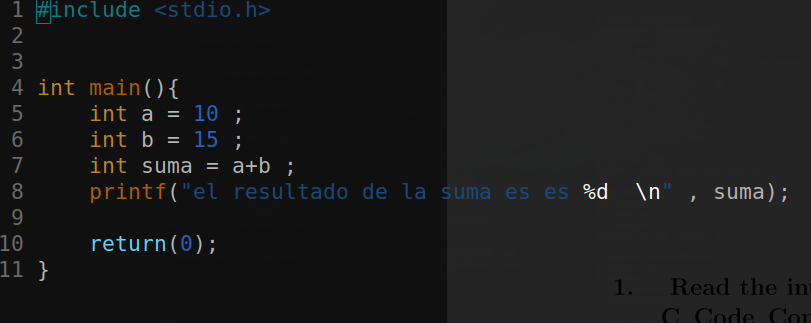
\includegraphics[width=1\linewidth]{codeforsum.png}
            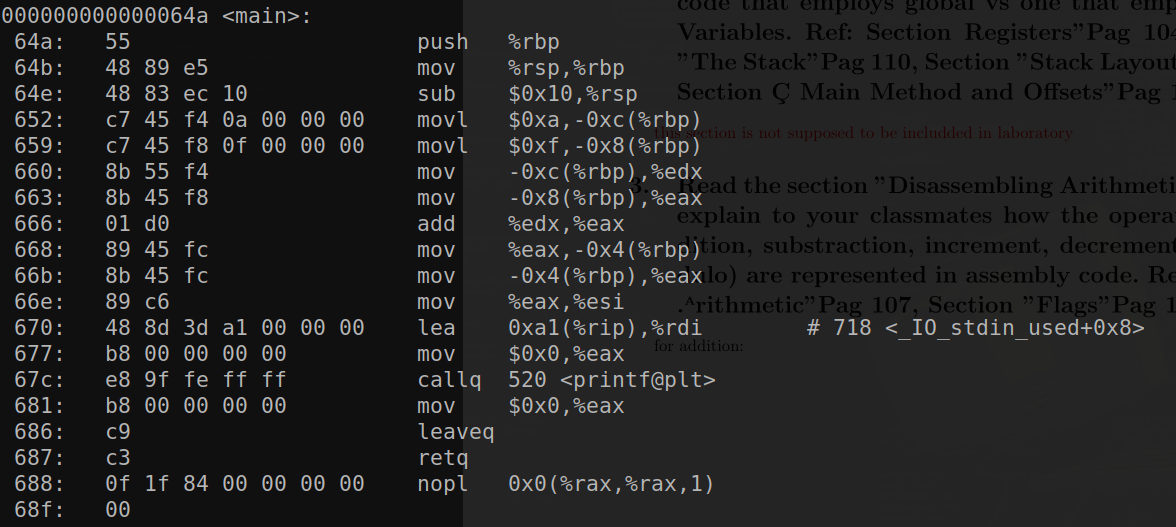
\includegraphics[width=1\linewidth]{sumadis.png}
            \caption{Code and disassembly for addition}
            \label{adfig}
        \end{figure}

        \newpage
        for substraction:
        this is the same as the addition operation, but, the code is replacing
        addition operation with substraction operation in line $ 663  $ .
        \begin{figure}[h!]
            \centering
            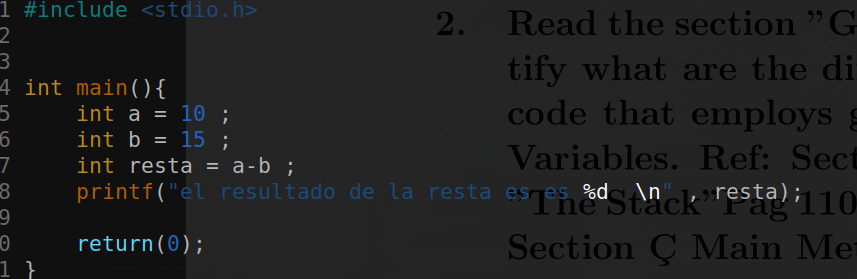
\includegraphics[width=1.0\linewidth]{codeforres.png}
            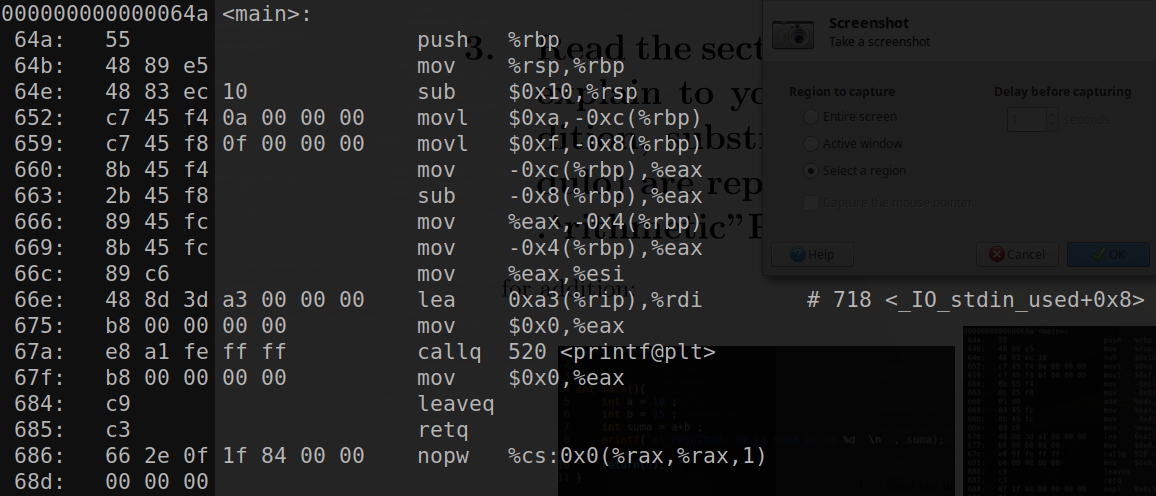
\includegraphics[width=1.0\linewidth]{resdis.png}
            \caption{Code and disassembly for substraction}
            \label{subfig}
        \end{figure}


        \newpage
        for increment:
        first, in line $ 652  $ we can see that is adding the value $ 0xa  $
        into a register, this value, is $ 10  $  , then its adding $ 0x1  $
        into the same register, this means that is adding 1 and now the value
        of this register is $ 11  $ .
        \begin{figure}[h!]
            \centering
            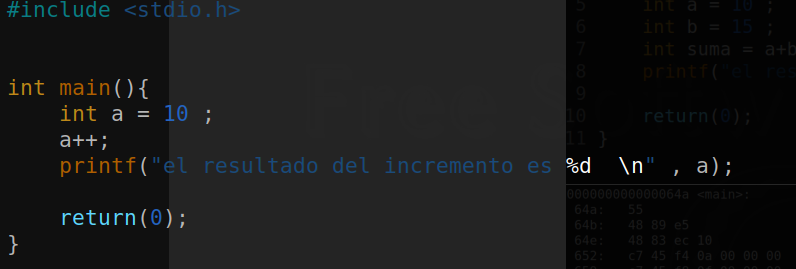
\includegraphics[width=1.0\linewidth]{codeinc.png}
            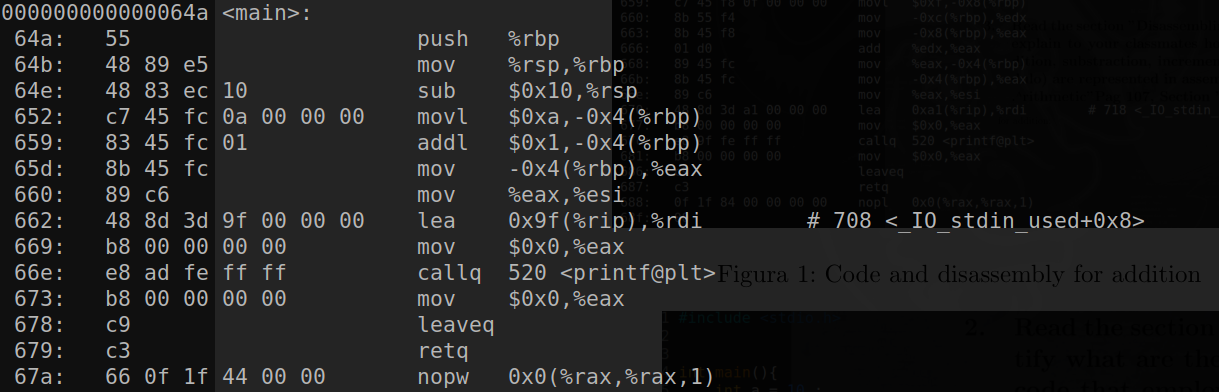
\includegraphics[width=1.0\linewidth]{incdis.png}
            \caption{Code and dissasembly for increment}
            \label{incfig}
        \end{figure}


        \newpage
        for decrement:
        is exactly the same as increment, but now, he es substracting instead
        of adding $ 0x1  $ value into the register.
        \begin{figure}[h!]
            \centering
            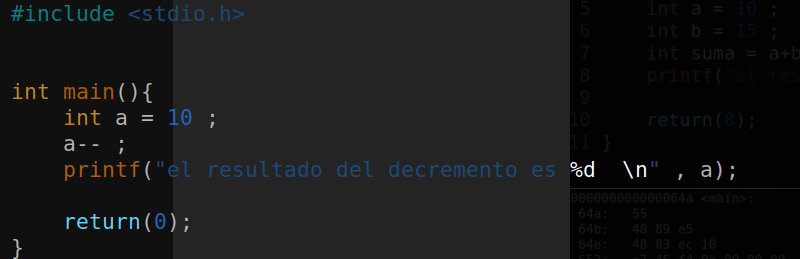
\includegraphics[width=1.0\linewidth]{deccode.png}
            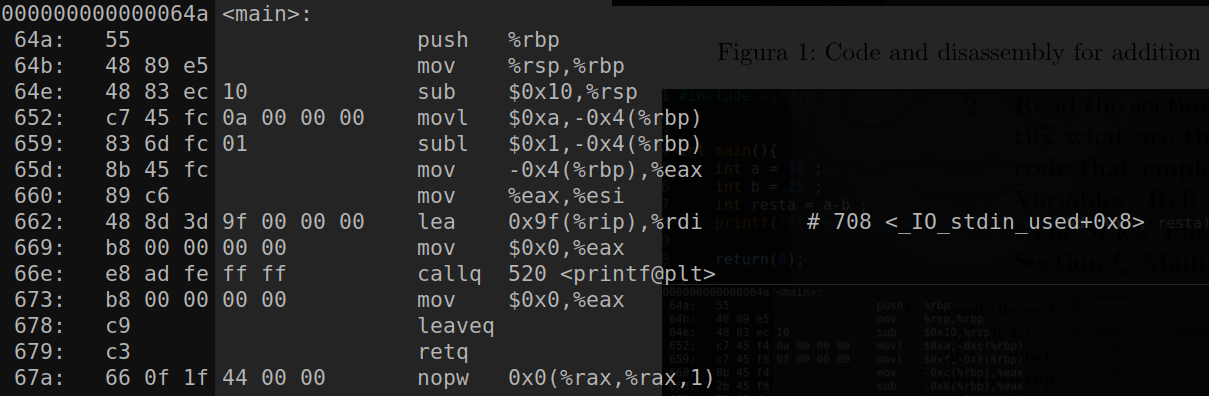
\includegraphics[width=1.0\linewidth]{decdis.png}
            \caption{Code and disassembly for decrement opperation}
            \label{figdec}
        \end{figure}

        \newpage
        for modulo:
        is actually the same as addition and substraction, but the opperation $
        idivl  $ stands for division, the result of this divion is going to
        store the residue in the designer register.
        \begin{figure}[h!]
            \centering
            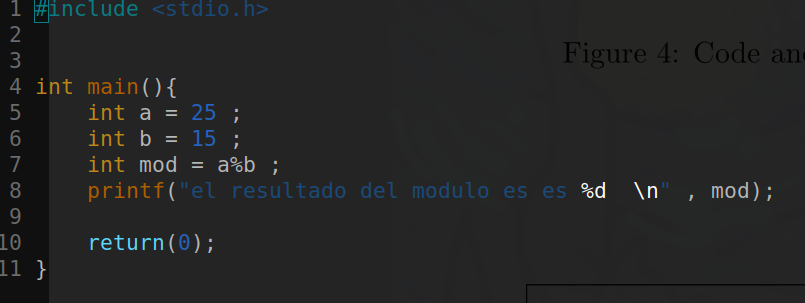
\includegraphics[width=1.0\linewidth]{modcode.png}
            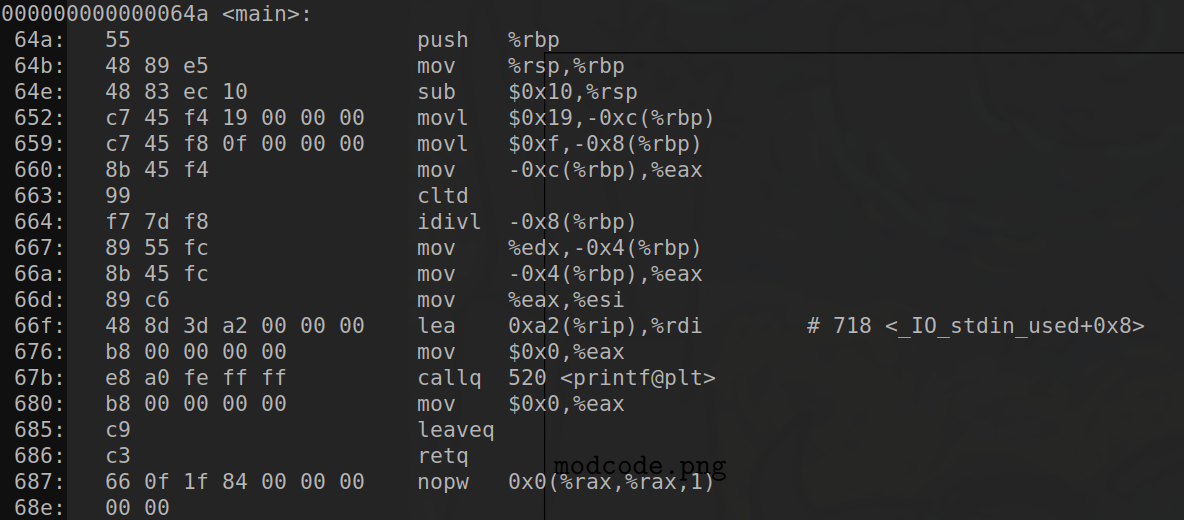
\includegraphics[width=1.0\linewidth]{moddis.png}
            \caption{Code for modulo}
            \label{figmode}
        \end{figure}








    \section{Q4: Read the section "Recognizing if Statements" and explain to
        your classmates how to recognize an if/else structure in assembly code.
        Ref: Section "Conditionals" Pag 113, Section "Branching" Pag 113}


%
%        % ====| RESPUESTA ACÁ |==== %
%
%    \section{Q5: Read the section "Recognizing Nested if Statements" and
%        explain to your classmates how to recognize a "Nested IF" structure in
%        assembly code.Ref: Section "Conditionals" and "Branching" Pag 113}
%
%        % ====| RESPUESTA ACÁ |==== %
%
%    \section{Q6: Read the section "Recognizing Loops" and explain to your
%        classmates how to recognize a FOR structure in assembly code.
%        Ref: Section "Conditionals" and "Branching" Pag 113}
%
%        % ====| RESPUESTA ACÁ |==== %
%
%    \section{Q7: Read the section "Recognizing Loops" and explain to your
%        classmates how to recognize a WHILE structure in assembly code.
%        Ref: Section "Conditionals" and "Branching" Pag 113}
%
%        % ====| RESPUESTA ACÁ |==== %
%
%    \section{Q8: Read the section "Understanding Function Call Convenstions"
%        and explain to your classmates how to recognize a "function call" in
%        assembly code.
%        Ref: Section "Function Calls" Pag 110. Section "Stack Layout" Pag 111. }
%
%        % ====| RESPUESTA ACÁ |==== %
%
%    \section{Q9: Read the section "Analyzing switch Statements" and explain to
%        your classmates how to recognize a switch structure in assembly code.}
%
        % ====| RESPUESTA ACÁ |==== %







    %=======================NOTES ENDS HERE===================%

    % bib stuff
    \nocite{*}
    \addtocontents{toc}{{}}
    \addcontentsline{toc}{section}{\refname}
    \bibliographystyle{plain}
    \bibliography{../Bibliography}
\end{document}
